\documentclass[11pt,a4paper]{article}

\usepackage[margin=2.5cm]{geometry}
\usepackage{booktabs}
\usepackage{graphicx}
\usepackage{amsmath}
\usepackage{xcolor}
\usepackage{caption}
\usepackage{float}
\usepackage[hidelinks]{hyperref}
\usepackage{enumitem}

\emergencystretch=2em

\definecolor{deepblue}{RGB}{31,78,99}
\definecolor{midblue}{RGB}{46,139,168}

\newcommand{\cat}[1]{\texttt{#1}}
\newcommand{\unreached}[0]{\textcolor{red!70!black}{\textbf{never reached}}}

\title{\textbf{The Five Reached Categories}\\
\large --- and Why Two Could Never Be Reached\\[2pt]
\normalsize Companion to \emph{Do Simulated Conversations Reproduce Real Agent Failures?}}
\author{Eduardo Fernandez Salazar\\
\small Imperial College London \;\textperiodcentered\; MSc Artificial Intelligence \;\textperiodcentered\; Pulpoo / Samsung Polanco}
\date{29 July 2026}

\begin{document}
\maketitle

\begin{abstract}
\noindent
The main comparison report presents all seven reachable failure categories side by side and reports
71\% category coverage (5/7). This companion document isolates the other half of that result: it
explains, mechanistically, why the two uncovered categories --- \cat{comprehension} and
\cat{data\_gap} --- \emph{cannot} appear under the current simulation design at any scale, and it
re-presents the real-vs-simulated comparison restricted to the five categories the simulator
actually reached, with percentages renormalised over that five-category support. Two results
follow. First, the unreached categories are structural zeros, not sampling artefacts: across
independent batches of 10 to 1{,}000 simulated conversations and a pooled corpus of 2{,}560, both
categories occur exactly zero times, and coverage is flat at 71\% from $N{=}50$ onward. The causes
are identifiable design idealisations --- over-cooperative LLM personas that rephrase instead of
repeating (extinguishing the behavioural signal that defines a comprehension failure), and a fully
seeded fake database in which missing-data failures are logically impossible. Second, on the ground
where both corpora can compete, the correspondence is substantially better than the headline
figure suggests: the Jensen--Shannon divergence between the renormalised five-category failure
distributions is \textbf{0.099 bits}, versus 0.239 bits on the seven-category support --- more than
half of the headline divergence is attributable to the two structural zeros rather than to the
simulator mis-ranking the failure modes it can express.
\end{abstract}

\section{Purpose and provenance}

The main report (\texttt{docs/results/real\_vs\_sim/REPORT.md}) is left unchanged. This document
does two things that report deliberately does not:

\begin{enumerate}[nosep]
  \item It explains, in depth, why two of the seven reachable categories ---
        \cat{comprehension} and \cat{data\_gap} --- never appeared in simulation, at any scale,
        and why this is a structural property of the simulation design rather than bad luck or
        insufficient sampling.
  \item It re-presents the comparison restricted to the five categories the simulator actually
        reached, with percentages renormalised over that five-category support, so the two corpora
        are compared like-for-like on the ground where both can actually compete.
\end{enumerate}

\noindent
All numbers derive from the scorer-parity comparison
(\texttt{real\_vs\_sim.json}, taxonomy \texttt{1.0-frozen-2026-07-14}, failure threshold
\texttt{min\_score}${}=3.0$): 1{,}299 real production conversations (376 failures, 28.9\%) versus
390 live-agent simulated conversations (82 failures, 21.0\%), both labelled by the
\emph{identical} rule-based production scorer, with no LLM in the scoring loop. Scale evidence
comes from the scale study (seven independent batches, $N=10$ to $1{,}000$, pooled 2{,}560).
Charts are generated by \texttt{debugger-platforn/reached\_only\_charts.py}.

\section{Quick recap: the seven categories}

The frozen taxonomy contains eight production-observable failure categories. One,
\cat{delivery\_infra} (WhatsApp message-delivery and infrastructure failures, 14 real
occurrences), is \emph{unreachable by design}: the simulator talks to the agent over HTTP and has
no WhatsApp transport layer, so nothing exists that could fail that way. It is excluded from all
coverage claims up front, leaving the seven reachable categories of Table~\ref{tab:seven}.

\begin{table}[H]
\centering
\small
\begin{tabular}{llr}
\toprule
category & what it means & real failures flagged \\
\midrule
\cat{loop\_stall} (infinite\_loop) & agent repeats itself; conversation circles & 256 (68.1\%) \\
\cat{resolution} & understood but could not resolve; user demanded a human & 221 (58.8\%) \\
\cat{comprehension} & agent did not understand what the user needed & 153 (40.7\%) \\
\cat{data\_gap} & backend/tool data missing or incomplete & 48 (12.8\%) \\
\cat{hallucination} & agent fabricated information; customer pushed back & 13 (3.5\%) \\
\cat{missed\_escalation} & frustrated user; agent failed to hand off & 11 (2.9\%) \\
\cat{silent\_abandonment} (premature\_exit) & conversation died without closure & 9 (2.4\%) \\
\bottomrule
\end{tabular}
\caption{The seven reachable categories. Percentages are of the 376 failed real conversations;
categories are multi-label, so they sum to more than 100\%.}
\label{tab:seven}
\end{table}

Of these seven, the simulator reproduced five. The two it never reproduced are not fringe
categories: together they account for the first and fourth most common real failure modes, and
\cat{comprehension} alone is present in over 40\% of real failures. Understanding \emph{why} they
never show up matters more than the coverage number itself.

\section{The two categories that were never reached}

\begin{figure}[H]
\centering
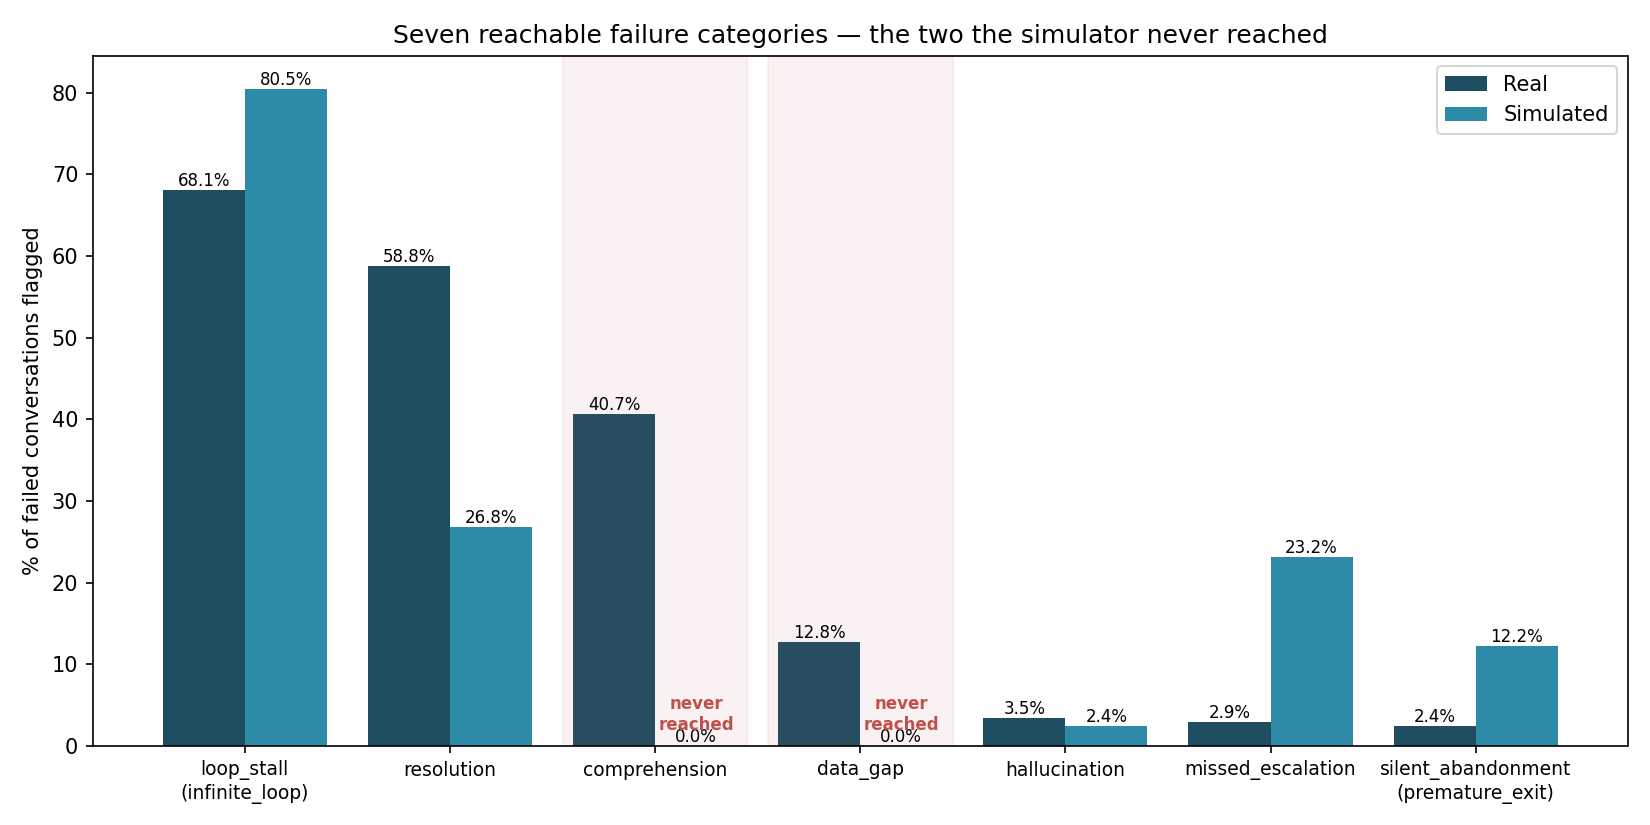
\includegraphics[width=\textwidth]{reachability_overview.png}
\caption{All seven reachable categories, real vs.\ simulated flag rates among failures. The two
categories the simulator never reached are shaded; their simulated bars are exactly zero at every
scale tested.}
\label{fig:overview}
\end{figure}

\subsection{\cat{comprehension}: the simulated customers are too polite, too clear, and too
cooperative}

\paragraph{What the category captures in production.}
A comprehension failure is flagged when the \emph{customer's} behaviour signals that the agent did
not understand them --- most observably, the customer repeating or re-sending essentially the same
request because the agent answered something else. Real WhatsApp customers produce this signal
constantly: fragmented messages, slang and regional abbreviations, mixed topics in one message,
typos, single-word messages (``precio??''), follow-ups of ``?'' or ``hola?'' when ignored --- and,
crucially, when the agent misunderstands them, they repeat themselves verbatim, often with
escalating frustration.

\paragraph{Why the simulator cannot produce it.}
The simulated customers are themselves LLM personas, and LLM-generated users are systematically
\emph{over-cooperative}. When the agent under test gives a confusing or off-target answer, the
persona does not do what a real annoyed customer does (paste the same message again, or reply
``no, eso no es lo que pregunt\'e''). Instead it behaves like a model trained to be helpful: it
\emph{rephrases} its request more clearly, adds context, answers the agent's clarifying questions
patiently, and generally repairs the conversation. Grammatically clean, well-structured,
single-intent messages are also exactly the inputs the agent under test comprehends best --- so
persona politeness attacks the failure mode from both sides: it makes misunderstanding less likely
to occur, and when it does occur, it erases the behavioural evidence (verbatim repetition) that the
scorer needs to flag it. This over-cooperative simulated-user effect is a documented phenomenon in
the user-simulation literature (the ``Lost in Simulation'' line of work), not something unique to
this project.

There is a secondary, telemetry-side reason the reachability matrix records this category as only
\emph{partially} reachable even in principle: part of the production comprehension signal comes
from intent/confidence telemetry emitted by the production stack, which does not exist in the
simulation harness. The customer-repeat behavioural signal \emph{is} observable in simulation ---
it simply never fires, for the reasons above.

\paragraph{In one sentence.} Real customers get confused and grind; LLM personas clarify and
cooperate, so the behaviour that \emph{defines} a comprehension failure never happens.

\subsection{\cat{data\_gap}: a fully seeded fake database has no gaps}

\paragraph{What the category captures in production.}
A data-gap failure occurs when the agent does everything right conversationally but the
\emph{backend} lets it down: the customer's record is missing, an order is not in the system yet,
a field is stale or empty, a lookup returns nothing. The failure originates in the data
environment, not in the agent's reasoning. In the real corpus this is 12.8\% of failures --- real
CRMs are messy.

\paragraph{Why the simulator cannot produce it.}
The simulation environment runs the agent against a single, deliberately \emph{fully seeded} fake
customer database, built so that every tool call the agent might make has a complete, well-formed
answer --- which is exactly what you want when the object under test is the agent's behaviour, and
exactly what makes data-gap failures \emph{logically impossible}. Every lookup succeeds; every
record exists; every field is populated. There is no incomplete state anywhere in the environment
for the agent to stumble over, so no quantity of simulated conversations can surface this
category. The failure mode lives in the environment, and the environment was built without it.

\paragraph{In one sentence.} You cannot discover missing-data failures in a world where no data is
ever missing.

\subsection{Why this is structural, not a sampling accident}

If the two categories were merely \emph{rare} in simulation, running more simulations would
eventually find them. The scale study rules this out. Seven independent batches were run at
$N = 10, 50, 100, 200, 400, 800, 1000$, plus a pooled corpus of 2{,}560 conversations:

\begin{itemize}[nosep]
  \item \cat{comprehension} occurrences in simulation: \textbf{0 at every $N$, and 0 in the pooled
        2{,}560};
  \item \cat{data\_gap} occurrences in simulation: \textbf{0 at every $N$, and 0 in the pooled
        2{,}560};
  \item category coverage sits at exactly 5/7 (71\%) from $N{=}50$ through $N{=}1000$ --- the
        curve saturates almost immediately and never moves again. Scaling grows failure
        \emph{volume} linearly but adds no new failure \emph{kinds}.
\end{itemize}

\noindent
A $100\times$ increase in simulation budget changed nothing, which is the empirical signature of a
structural ceiling: the generating process for these two categories is \emph{absent}, not
undersampled. Buying more of the same simulations buys zero additional coverage; reaching these
categories requires \emph{different} simulations (Section~\ref{sec:future}).

\section{The five reached categories, renormalised}

\subsection{How to read the percentages}

The main report expresses each category as a share of \emph{failed conversations} (multi-label:
one failed conversation can carry several category flags, so columns sum to more than 100\%). That
framing is kept in Figure~\ref{fig:rates}. For the composition comparison, the percentages are
\textbf{renormalised over the five-category support}: each category's flag count is divided by the
total number of flags across the five reached categories (real: 510 flags across 376 failures;
simulated: 119 flags across 82 failures). This answers the question the raw rates cannot:
\emph{given only the failure kinds both worlds can express, how does the failure mass distribute
--- and does simulation distribute it the way reality does?} Zeroed-out categories no longer
distort the comparison, and the two corpora are judged only on ground where both can compete. The
renormalised shares describe the composition of \emph{flags}, not of conversations.

\begin{table}[H]
\centering
\small
\begin{tabular}{lrrrrrr}
\toprule
 & \multicolumn{2}{c}{real} & \multicolumn{2}{c}{simulated} & \multicolumn{2}{c}{5-category share} \\
\cmidrule(lr){2-3}\cmidrule(lr){4-5}\cmidrule(lr){6-7}
category & count & \% of failures & count & \% of failures & real & sim \\
\midrule
\cat{loop\_stall}          & 256 & 68.1 {\scriptsize(63.2--72.6)} & 66 & 80.5 {\scriptsize(70.6--87.6)} & \textbf{50.2\%} & \textbf{55.5\%} \\
\cat{resolution}           & 221 & 58.8 {\scriptsize(53.7--63.6)} & 22 & 26.8 {\scriptsize(18.4--37.3)} & \textbf{43.3\%} & \textbf{18.5\%} \\
\cat{hallucination}        &  13 &  3.5 {\scriptsize(2.0--5.8)}   &  2 &  2.4 {\scriptsize(0.7--8.5)}   & \textbf{2.5\%}  & \textbf{1.7\%}  \\
\cat{missed\_escalation}   &  11 &  2.9 {\scriptsize(1.6--5.2)}   & 19 & 23.2 {\scriptsize(15.4--33.4)} & \textbf{2.2\%}  & \textbf{16.0\%} \\
\cat{silent\_abandonment}  &   9 &  2.4 {\scriptsize(1.3--4.5)}   & 10 & 12.2 {\scriptsize(6.8--21.0)}  & \textbf{1.8\%}  & \textbf{8.4\%}  \\
\bottomrule
\end{tabular}
\caption{The five reached categories. Parenthesised ranges are Wilson 95\% confidence intervals on
the rate among failures. The final two columns renormalise flag counts over the five-category
support (real: 510 flags; simulated: 119 flags).}
\label{tab:five}
\end{table}

\subsection{Flag rates among failures --- the direct comparison}

\begin{figure}[H]
\centering
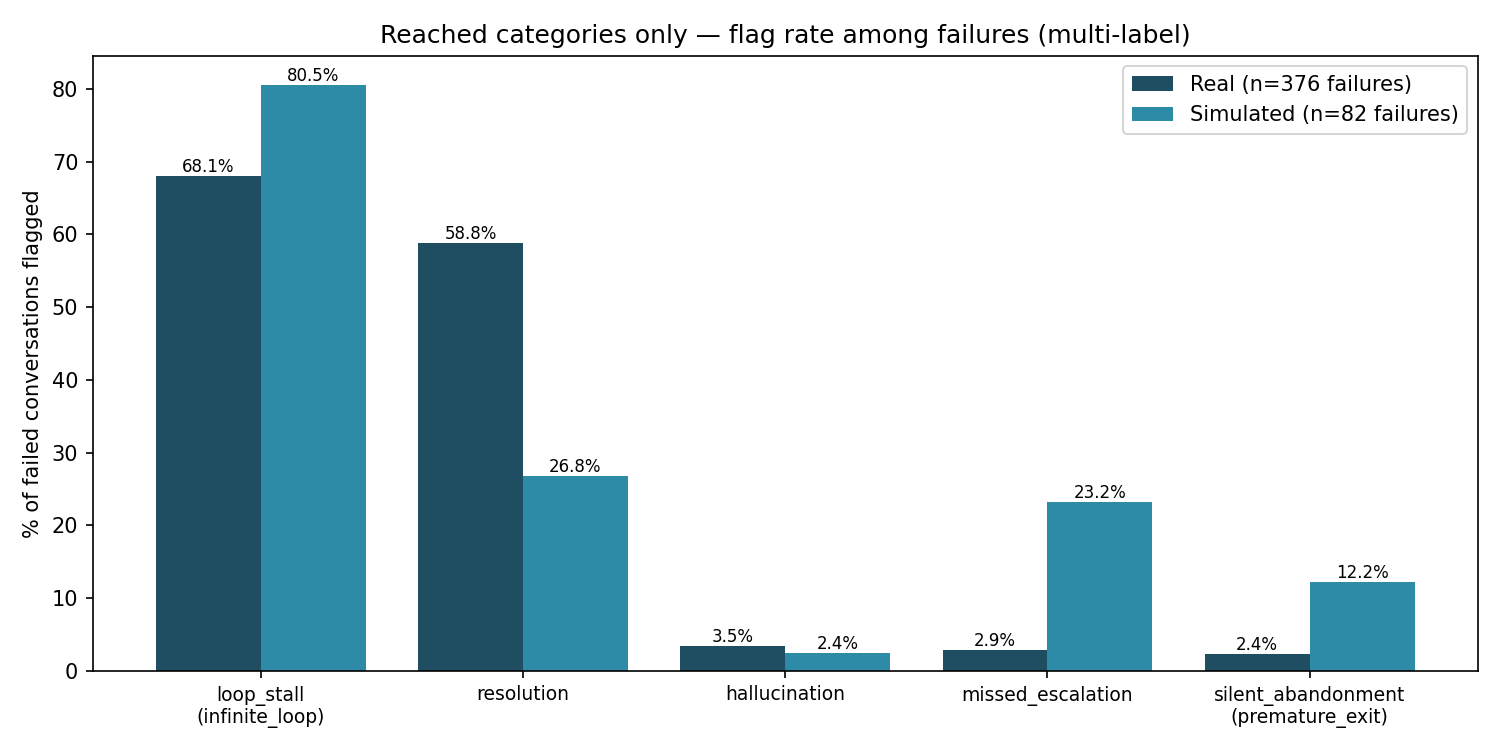
\includegraphics[width=0.95\textwidth]{reached_only_rates.png}
\caption{Flag rate among failed conversations for the five reached categories (multi-label). Real:
$n{=}376$ failures; simulated: $n{=}82$.}
\label{fig:rates}
\end{figure}

Reading Figure~\ref{fig:rates} category by category:

\begin{description}[leftmargin=1.2em, itemsep=3pt]
  \item[\cat{loop\_stall} --- reproduced, dominant in both worlds (68.1\% vs.\ 80.5\%).]
        The strongest correspondence result in the study: the single most common way the real
        agent fails --- getting stuck repeating itself --- is also the single most common way it
        fails under simulation, at comparable magnitude. Loop behaviour is a property of the
        \emph{agent} (its retry logic, its inability to break out of a clarification cycle), so it
        transfers into any environment that lets the conversation run long enough. The simulator
        slightly over-expresses it, plausibly because personas dutifully keep responding where
        real customers would have quit, giving loops more room to manifest.
  \item[\cat{resolution} --- reproduced but substantially under-produced (58.8\% vs.\ 26.8\%).]
        Resolution failures need a customer who insists on an outcome the agent cannot deliver and
        escalates the demand for a human. The same persona politeness that eliminates
        comprehension failures dampens this one: simulated customers accept partial answers and
        let the agent off the hook, where real customers keep pushing until the failure is
        undeniable. The category survives in simulation only because some scenario scripts
        explicitly direct the persona to demand things the agent cannot do.
  \item[\cat{hallucination} --- reproduced at close to the real rate (3.5\% vs.\ 2.4\%).]
        A small category in both worlds, and the simulated rate lands within sampling noise of the
        real one. Hallucination is agent-internal --- it does not depend on the customer being
        realistic --- which is exactly why it transfers cleanly.
  \item[\cat{missed\_escalation} --- reproduced but heavily over-produced (2.9\% vs.\ 23.2\%,
        ${\sim}8\times$).]
        The mirror image of the comprehension story: several test scenarios deliberately script
        frustrated personas who demand a human, precisely to probe the escalation path. The
        simulator therefore concentrates escalation pressure far above its natural production
        frequency. This is over-representation by test design, not a discovery error --- but it
        means the simulated rate measures how the agent handles \emph{engineered} escalation
        pressure, not how often that pressure arises organically.
  \item[\cat{silent\_abandonment} --- reproduced but over-produced (2.4\% vs.\ 12.2\%,
        ${\sim}5\times$).]
        Simulated conversations have hard turn budgets and personas with finite scripted patience,
        so conversations end without closure more often than in production, where customer
        abandonment is the tail event.
\end{description}

The overall pattern is coherent rather than random: \textbf{agent-internal failure modes (loops,
hallucination) transfer at close to their real magnitudes; customer-driven failure modes are
distorted in whichever direction the persona design pushes them} --- suppressed where personas are
too polite (resolution, and comprehension to the point of extinction), inflated where scenarios
script the pressure in (escalation, abandonment).

\subsection{Composition over the five-category support}

\begin{figure}[H]
\centering
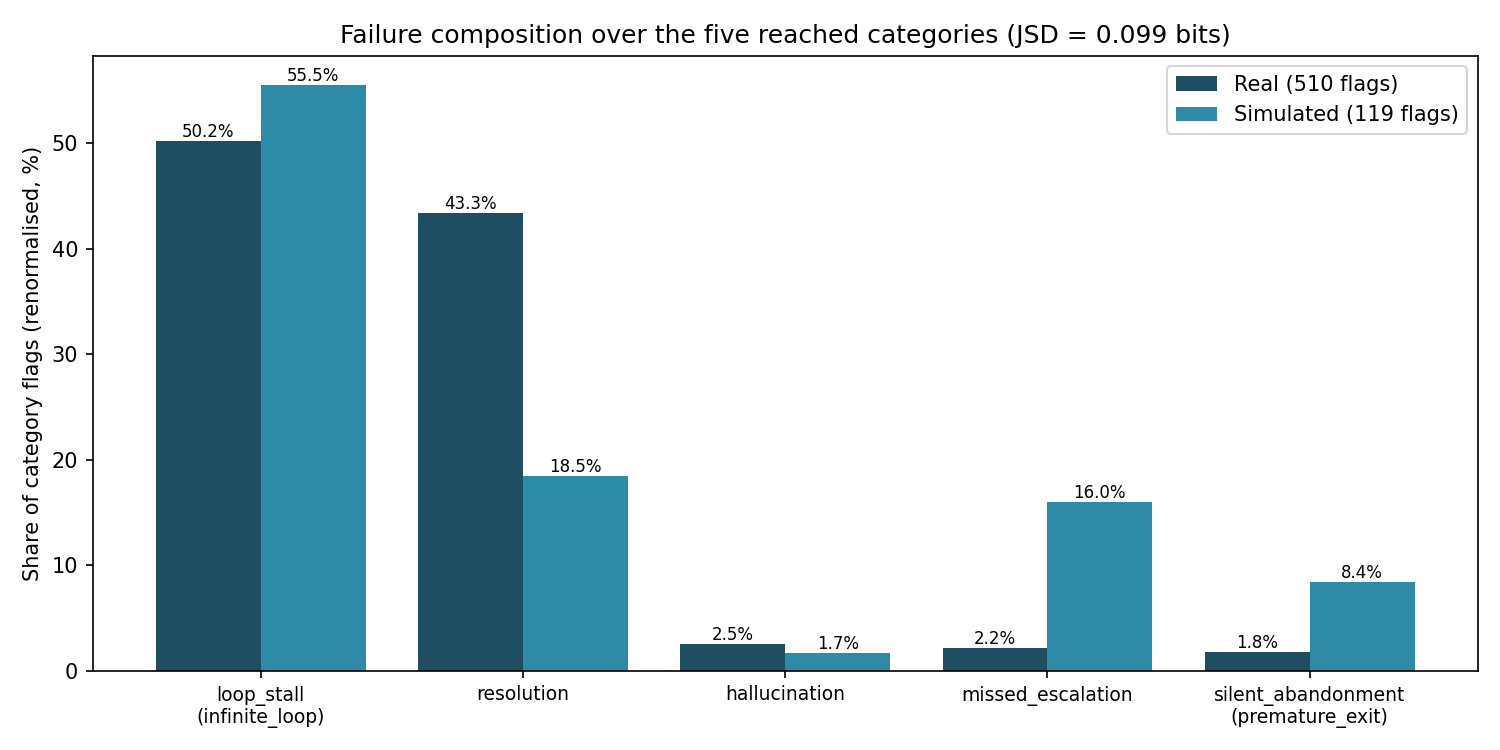
\includegraphics[width=0.95\textwidth]{reached_only_shares.png}
\caption{Failure composition renormalised over the five reached categories.
JSD${}=0.099$ bits.}
\label{fig:shares}
\end{figure}

\begin{figure}[H]
\centering
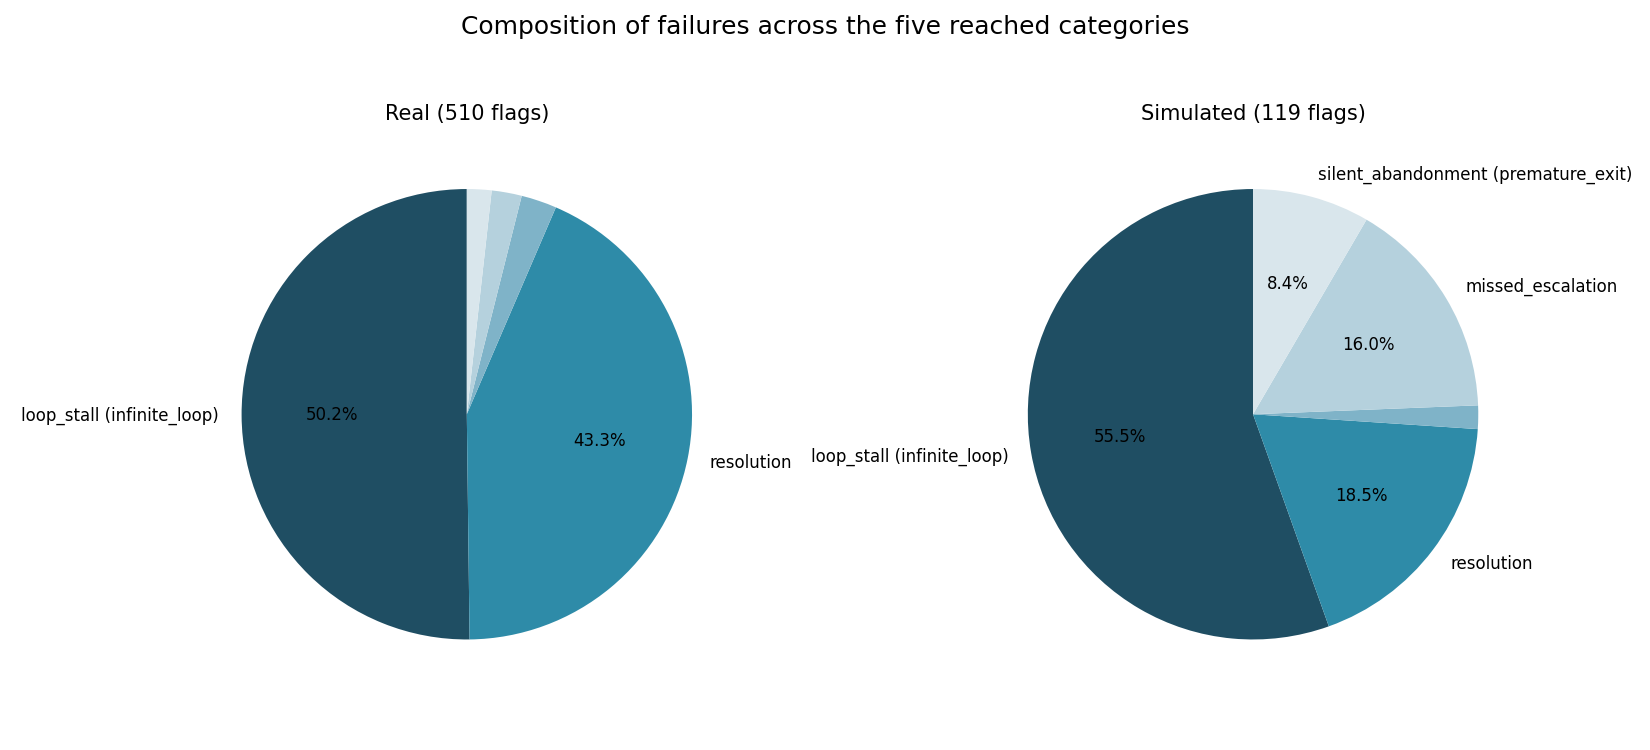
\includegraphics[width=\textwidth]{reached_only_composition.png}
\caption{The same renormalised composition as side-by-side pies. Real failure mass is essentially
two-mode (loops + resolution ${}=93.5\%$); simulation reproduces the loop mode at nearly the same
share but redistributes resolution mass into the scripted-pressure categories.}
\label{fig:pies}
\end{figure}

Renormalised, the real failure mass is essentially a \emph{two-mode distribution}: loops (50.2\%)
plus resolution (43.3\%) account for 93.5\% of all real flags on this support, with hallucination,
escalation, and abandonment sharing the remaining 6.5\%. The simulated distribution reproduces the
headline structure --- \cat{loop\_stall} is the plurality mode in both, at nearly the same share
(50.2\% real vs.\ 55.5\% simulated) --- but redistributes the rest: resolution's share drops from
43.3\% to 18.5\%, and the freed mass flows into the two scripted-pressure categories,
\cat{missed\_escalation} (2.2\% $\rightarrow$ 16.0\%) and \cat{silent\_abandonment}
(1.8\% $\rightarrow$ 8.4\%).

Quantitatively, the Jensen--Shannon divergence between the two renormalised five-category
distributions is \textbf{0.099 bits} --- versus \textbf{0.239 bits} on the seven-category
reachable support used in the main report (real split-half noise floor: 0.005). More than half of
the headline distributional divergence is therefore attributable to the two structurally-zeroed
categories, not to the simulator mis-ranking the failure modes it can actually express. On the
ground where both corpora can compete, the simulated failure distribution is much closer to
reality than the full-support number suggests --- though still an order of magnitude above the
noise floor, driven by the resolution-deficit / escalation-surplus swap described above.

\section{What this means for the overall claim}

The fair summary is neither ``the simulator found 71\% of failure categories'' alone, nor ``the
simulator missed the most common failure mode'' alone --- it is both, with the mechanism attached:

\begin{enumerate}[nosep]
  \item \textbf{What simulation is good at:} discovering and reproducing failures that live
        \emph{inside the agent} --- loops, inability to resolve, hallucination, escalation
        handling, premature termination. These it finds at $N$ as small as 50, with the dominant
        real mode (\cat{loop\_stall}) correctly identified as the dominant simulated mode, and
        with a five-support composition divergence (0.099 bits) a fraction of the full-support
        figure.
  \item \textbf{What this simulation design is blind to:} failures that require the
        \emph{customer} to be realistically difficult (\cat{comprehension}) or the
        \emph{environment} to be realistically broken (\cat{data\_gap}). These are exactly the
        ingredients the current design idealises away --- cooperative LLM personas and a fully
        seeded database --- and no quantity of additional simulation compensates, as the flat 71\%
        coverage curve from $N{=}50$ to $N{=}2560$ demonstrates.
\end{enumerate}

\noindent
The blindness is therefore \emph{diagnosable and, in principle, fixable} --- it points at specific
components (persona realism, environment seeding), not at simulation as a method.

\section{What it would take to reach them (future work)}
\label{sec:future}

\begin{description}[leftmargin=1.2em, itemsep=3pt]
  \item[\cat{comprehension}:] persona-realism interventions --- frustrated/impatient persona
        variants that repeat verbatim instead of rephrasing; typo/slang/code-switching noise
        injection into persona messages; fragmented multi-message inputs; explicit ``grinding''
        behaviour rules (if the agent's reply does not address the request, resend it). Each
        attacks the over-cooperativeness directly and would let the existing customer-repeat
        detector fire.
  \item[\cat{data\_gap}:] environment-side fault injection --- seed variants of the fake customer
        database with deliberately missing records, empty fields, and stale values, so agent tool
        calls can return the incomplete results that define the category. No new detector is
        required; the failure becomes observable the moment the environment permits it.
  \item[\cat{delivery\_infra}] (outside the seven; unreachable by design): would require
        simulating transport-level faults (dropped/duplicated/delayed messages), a harness feature
        rather than a persona or data feature.
\end{description}

\section{Caveats}

\begin{itemize}[nosep]
  \item The renormalised shares are shares of \emph{multi-label flags}, not of conversations; a
        conversation flagged for both loop and resolution contributes to both categories.
  \item The simulated failure sample is small (82 failures, 119 flags): simulated-side Wilson
        intervals are wide, and small-category shares (hallucination especially, $n{=}2$) are
        fragile.
  \item Both corpora are scored by the same rule-based scorer (scorer parity by construction, no
        LLM in the loop); human annotation of a sample --- and the resulting agreement figure ---
        is still pending, so all category counts inherit the scorer's precision.
  \item The JSD figures on different supports (0.099 on five categories vs.\ 0.239 on seven) are
        not directly comparable in a formal sense --- the support differs --- but the contrast is
        precisely the point: it isolates how much divergence the structural zeros contribute.
\end{itemize}

\vspace{1em}
\noindent\small
Charts and numbers: \texttt{docs/new\_coverage/} (source of record:
\texttt{docs/results/real\_vs\_sim/reached\_only/}); regenerate with
\texttt{cd debugger-platforn \&\& python3 reached\_only\_charts.py}. This document does not modify
the main report.

\end{document}
